\documentclass[a4paper,12pt]{article}

% Packages
\usepackage{graphicx}
\usepackage{amsmath}
\usepackage{geometry}
\usepackage{fancyhdr}
\usepackage{setspace}
\usepackage{titlesec}  % For title formatting
\geometry{margin=1in}
\setstretch{1.5}

% Header and Footer
\pagestyle{fancy}
\fancyhf{}
\fancyhead[L]{ECG Heartbeat Classification}
\fancyhead[R]{\thepage}

% Title Formatting
\titleformat{\section}{\normalfont\Large\bfseries}{\thesection}{1em}{}

% Cover Page
\title{
    \vspace{2cm} % Adjust vertical space
    
\includegraphics[width=0.55\textwidth]{logo-usth.jpg} \\ % Add your logo here (change "logo.png" to the actual filename)
    \vspace{1cm} % Adjust vertical space after the logo
    \textbf{\Huge Report submission\\ ECG heartbeat classification } \\
    \vspace{1cm} % Adjust vertical space
    \large Machine Learning in Medicine \\
    \vspace{0.5cm} % Adjust vertical space
    \large 27th February, 2025
}
\author{Thái Doãn Kiên}
\date{}

\begin{document}

% Title Page
\maketitle
\thispagestyle{empty}
\newpage

% Table of Contents
% Start page numbering from the Table of Contents
\setcounter{page}{1}  % Start counting from 1
\tableofcontents
\newpage

% 1. Objective or Summary
\section{Objective}
This report aims to explore the MIT-BIH Arrhythmia Dataset and provide systematic methods to tackle the classification task on this dataset. Multiple machine learning approaches have been derived to solve the problem \cite{Kachuee_2018} \cite{odugoudar2024ecgclassificationarrhythmiadetection}, proving the possibility of applying the approach in our course guide to this type of problem. Therefore, I decided to perform Explanatory Data Analysis on the dataset, thereby pin-pointing the direction I will make to apply some framework of Machine Learning on this typical ECG classification problem.

% 2. Problem Description
\section{Problem Description}
\subsection{Data class}
Firstly, I explore how the data is represented in the dataset, and propose my method to interpret and preprocess data before feeding it to the main pipeline to perform the prediction. After loading the dataset of ".csv" format provided by the author, I observe a total number of 87553 samples in the train set, attaching with 21891 samples in the test set, following a standard ratio of 8:2. Therefore, I decided to divide the test set further, to include another validation set with the intention to utilize in the process of evaluate the model in the training process. The test set will be used separately after a final model is derived to calculate some important metric score.

\begin{figure}[b]
    \centering
    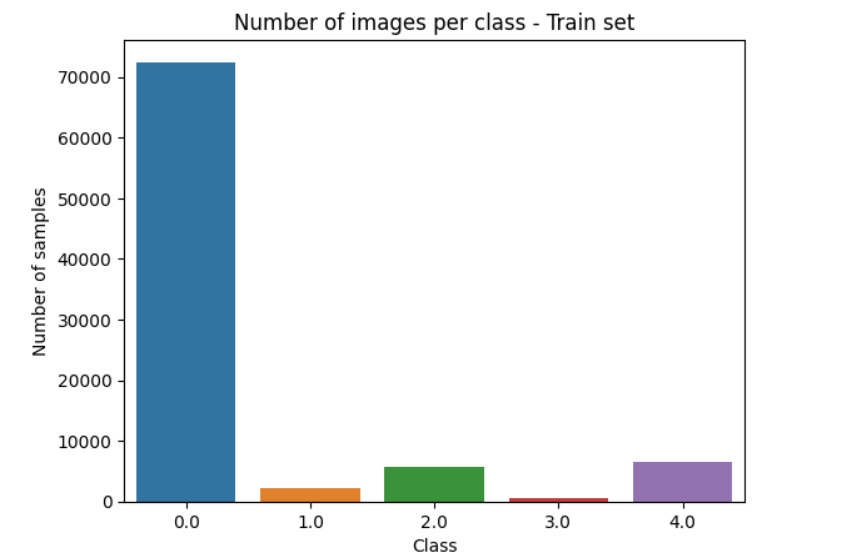
\includegraphics[width=0.5\linewidth]{sample_class.png}
    \caption{Number of samples in each class}
    \label{fig:fig1}
\end{figure}

\subsection{ECG Visualization}
I use Matplotlib to visualize the behaviour of each class ECG case. For an unspecialized human being to discriminate between each class is nearly impossible, as we need to iterate through hundreds of cases to recognize the pattern in each class. This tedious and requirement-specific task \cite{9397163} is thereby potential for an algorithmic mechanism to replace and provide an automatic pipeline to classify each case. 
\begin{figure}[h!]
    \centering
    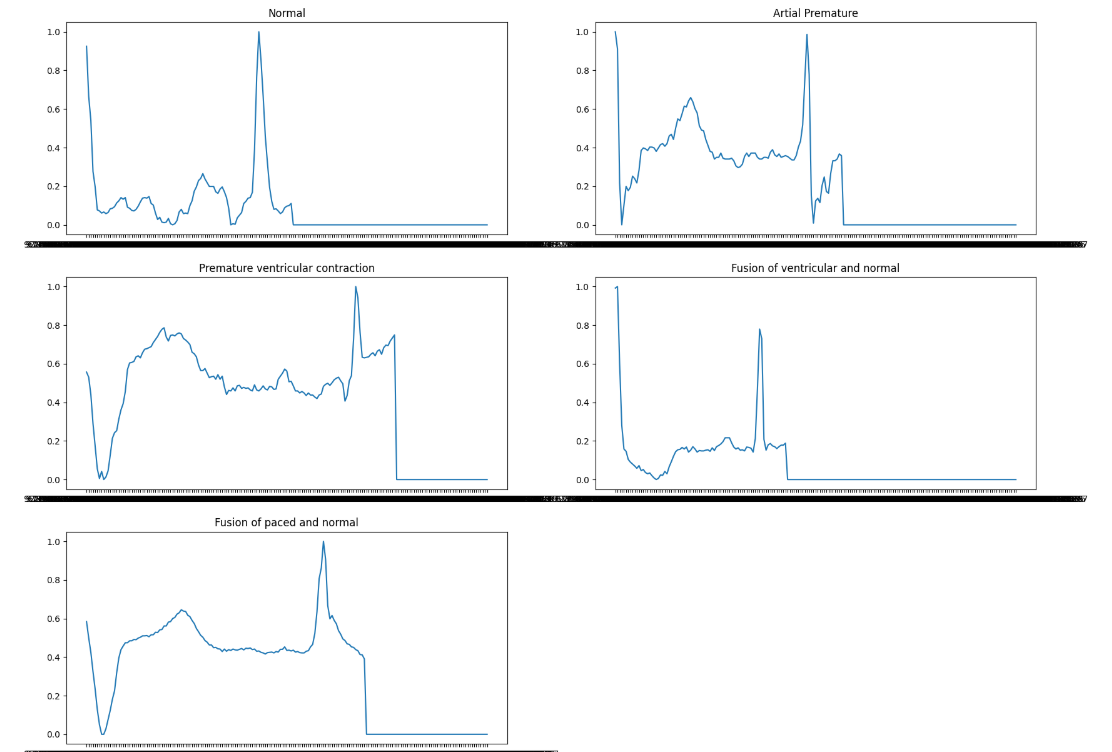
\includegraphics[width=0.5\linewidth]{ecg_visual.png}
    \caption{ECG visualization of all classes, including Normal, Artial Premature, Premature ventricular contraction, Fusion of ventricular and normal and Fusion of paced and normal}
    \label{fig:fig2}
\end{figure}




% 3. Methodology/Design Procedures
\section{Methodology}
\begin{figure}[h!]
    \centering
    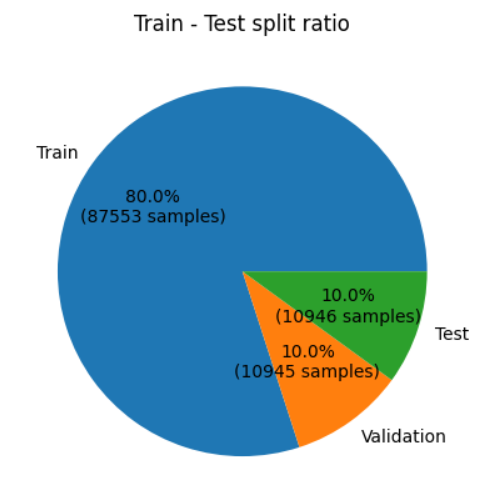
\includegraphics[width=0.5\linewidth]{train_split.png}
    \caption{Train-Test split of the dataset}
    \label{fig:fig3}
\end{figure}
\subsection{Train - Test split}
In this study we also make use of the test and validation dataset so as to ensure the integrity of the test dataset only taken for testing the final model in some major metrics. Therefore we split the test set into half and take the other half as our validation dataset.

\subsection{Handle data imbalance}
As we can obviously see in the dataset, the class samples are heavily imbalanced, as more than 70k samples belong to the "Normal" class ("0.0" denoted for Normal). Therefore, it is necessary to provide a baseline re-weighting method to balance the dataset. The weight of each class following this formula:
$$ weight_i = \frac{\sum_isamples_i}{samples_i}$$ for i corresponds to class.\\
We add the weighting loss into the sampling method called weighted random sampler. This sampling method ensures for each data batch, the probability of appearing an instance of class $i$ will be multiply by $weight_i$. 
\begin{figure}[h!]
    \centering
    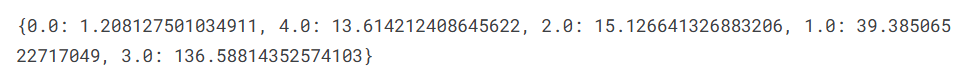
\includegraphics[width=1\linewidth]{imbalance.png}
    \caption{Weight for each class in the dataset. The 3.0 class has a multiplier weight of ~ 136.5}
    \label{fig:fig4}
\end{figure}
We observe a huge distance (more than 100 times) between class 1.0 and class 3.0. This suggests that the recommended sampler should not be enough. We could generate more synthetic data to make our model generalize better, which in this study we shall not perform in the scale of our labwork.

\subsection{LSTM}
My first thought within this task is that there is a tight time relationship among data features. Therefore, the problem can be viewed as a time-series representation, where some major advancements has been made. Long-short Term Memory (LSTM) \cite{6795963} has been widely recognized as a game-changer architecture for sequence-to-sequence modeling. It surpassed and harmonized the prior precedent Recurrent Neural Network (RNN) by introducing multiple gating mechanisms to limit the gradient vanishing/exploding problem. Therefore, I apply the architecture of LSTM to this problem

I design a fairly basic LSTM architecture for faster experiments and hyper-parameter tuning. The model includes 2 LSTM layers of (input size, 128) and (128, 64), each processing the data of sequence length 1. After that a simple dense layer is connected with dimension 64 to output the same number of classes. The experiment is conducted with Adam optimizer of learning rate 1e-3, loss function Cross Entropy and a learning rate scheduler of factor 0.5 whenever 2 validation steps consecutively were not improved.


% 4. Measurement/Testing Results
\section{Results}
For the LSTM model, we 

\begin{figure}[h!]
    \centering
    \includegraphics[width=0.8\textwidth]{example-image} % Example of adding a figure
    \caption{Test results for circuit 1}
    \label{fig:circuit1}
\end{figure}

% 5. Analysis and Discussion
\section{Analysis and Discussion}
Interpret the results obtained. Compare them with theoretical values, explain discrepancies, and discuss their significance.

% 6. Recommendations/Conclusions
\section{Conclusions}
Provide conclusions based on the results and discuss any recommendations for improvements, future work, or alternative solutions.

\newpage
% Bibliography (if required)
\bibliographystyle{plain}
\bibliography{references}  % Add a .bib file if you have references

\end{document}
